%!TEX root = ../projecto.tex
\section{Basic Concepts} % (fold)
\label{sec:basic_concepts}
In this section we will start by generally describing what Clustering is and how it works at subsection \ref{sub:clustering}, then at subsection \ref{sub:self_organizing_maps} it will be outlined how Self-organizing \cite{Kohonen1990}maps function, which is the Document Clustering algorithm used on this project.


\subsection{Document Clustering} % (fold)
\label{sub:clustering}
Document clustering is an optimal division of data into cathegories without prior knowledge of the data that is being organized, based only on the similarity between documents. Due to the fact that no prior knowledge of the date has to be known Document Clustering is labeled as Unsupervised Machine Learning.

Yuan-Chao Liu et Al \cite{Liu2012b} described that Document Clustering can be used to a variety of Computer Science fields, such as:
\begin{itemize}
  \item Natural Language Preprocessing.
  \item Automatic Sumarization.
  \item User preference mining.
  \item Improve Text classification results.
\end{itemize}

In regard to document categorization there are two main types of Document Clustering, Hard Clustering and Soft Clustering. In Hard Clustering one document can only belong to one cluster, while in Soft Clustering one document can belong to multiple clusters. 

In regard to document categorization \citet{Springorum1998} performed hard and soft clustering with SOMs \citep{Kohonen1990} while identifying polysemous German Propositions. They used regular SOMs to create multiple hard clusters and used Centroid-Based or Preposition-based softening to create Soft Clusters from the Hard Clusters.

The general mathematical description of Document Clustering can be seen in \ref{fig:1_Text_Clustering_Main_Framwork}
\begin{figure}
  \begin{center}
    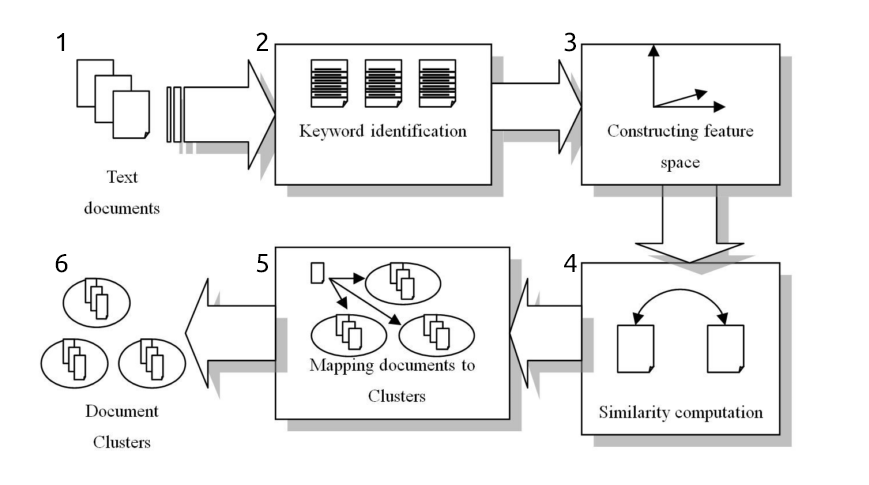
\includegraphics[width=12cm]{images/1_Text_Clustering_Main_Framwork.png}
  \end{center}
  \caption{ Text Clustering Main Framework from \citet{Dozono2012} }
  \label{fig:1_Text_Clustering_Main_Framwork}
\end{figure}
In the first step a data set must be provided in order to cluster the documents. 
The second step "Keyword identification" is where non relevant words are removed from the documents. \citet{Kang2003} proves that keyword removal improves clustering. Another way to extract features is to differentiate text features by analizing the document corpora. For example if the dataset is composed from HTML or XML documents it is possible to identify more relevante features due to the characteristics of the markup. In \ref{sub:topic_detection_on_twitter} it will be described twitts characteristics as a document and in \ref{sec:architecture} how feature extraction will be implemented on this project.
"Constructing the Feature Space" is characterized by converting the keywords of each document into vectors, the most common algorithm used for this task is SVM (Support Vector Machines). In SVM each vector dimension means one detected key word and each document is represented by the vector of keywords in the feature space. This process and keyword removal is described in Figure \ref{fig:2_svm}.
Due to the way documents are represented in SVM it is normal that vectors become very large and full of zeros ( keywords not present) and it is needed to use sparse vectors to represent the documents in a more efficient way.

\begin{figure}
  \begin{center}
    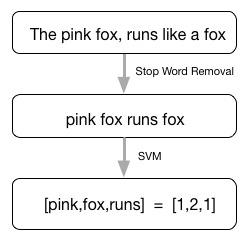
\includegraphics[width=5cm]{images/2_svm.jpg}
  \end{center}
  \caption{ Stop word removal and transformation to Vector Space Model }
  \label{fig:2_svm}
\end{figure}

Dimensional reduction is done after the construction of the vector space model, in order to reduce the size of the vector space. There are two main ways to do this PCA (Principal Component Analysis) and LSI (Latent Semantic Indexing). PCA calculates the k eigenvectors of the co-variance of the document matrix, which reduces the size of the matrix to k. LSI (Latent Semantic Indexing) works just like PCA but the eigenvectors are calculated directly from the document matrix.

There are two main strategies for Document Clustering, Complete strategie where the data set does not change and Incremental where initial number of document can increase by adding new documents. After a new document is added it can be merged into a existing cluster, or can be separated as a new category. While adding new documents it might be needed to re run the clustering algorithm. 

After the algorithm converges, cluster similarity can be calculated in multiple ways:
\begin{itemize}
  \item Shortest Distance Method: Shortest distance between two members of different clusters.
  \item Longest Distance Method: Longest distance between two members of different clusters.
  \item Group Average Method: The average distance between all elements of both clusters.
  \item Centric Method: The distance between the center of two clusters.
\end{itemize}

There many clustering algorithms, here we will focus on the three most popular.K-means works by randomly selecting k documents as the cluster centroids, then assign each document to the nearest centroid, and finally recalculate the the centroid with new added documents. The algorithm should be executed until convergence which reflects in the centroids stop changing. K-means has the advantage that the number of centroids must be selected before starting the algorithm.
AHC or Agglomerative Hierarchical Clustering is hierarquical clustering algorithm where clusters have sub-clusters which have subclusters. Like K-means it is also a simple algorithm that starts by calculating the similarity matrix, then each document is seen as a cluster and finally merge the nearest two clusters into one and update the similarity matrix. The algorithm ends when there is only one cluster or due to clustering entropy.An AHC classic example is species taxonomy where species have subspecies which have subspecies, etc.
Lastly there is Self-organizing Maps introduces by \citep{Kohonen1990} which will be used in the thesis and will be detailedly described in the next subsection \ref{sub:self_organizing_maps}.


% subsection clustering (end)

\subsection{The Self-organizing Map} % (fold)
\label{sub:the_self_organizing_map}

The Self-organinzing map, or for short SOM is a kind of recurrent artificial neural network that as the desired property of topology preservation which mimics the way cortex of high developed animals brains work.

SOMs work similar to the way that is thought that the human brain works by having a set of neurons that through learning experience specialize in the identification of certain types of patterns. These so called neurons are responsible for categorizing input patterns for which they are responsible. Nearby neurons will be organized by similarity which will cause that similar patterns will activate in similar areas of the SOM.
With a topology preserving mapping, SOM organizes the information spatially where similar concepts are mapped to adjacent areas.
Neurons are displayed in an n dimensional grid, generally rectangular, but other dimensions are possible like hexagonal or octagonal.  The grid of neurons, also called output space can be divided in neighborhoods where neurons responsible for the same kind of input reside.
In SOM neurons will have the same amount of coefficients as the input patterns and can be represented as vectors through the SVM model described earlier in section \ref{sub:clustering}.

Before describing the algorithm it is important to define two key aspects of the SOM, the learning rate and quantization error. The learning rate is a function that will be decreased in order to converge to zero, it will be applied to winning neurons and their neighbors in order for them to move toward the corresponding input pattern. Quantization Error is the distance between a given input pattern and the associated winning neuron, it describes how well neurons represent the input pattern.
The learning phase is characterized by the training algorithm, which works the following way:
\begin{itemize}
  \item Neurons can be initialized randomly or it is possible to select initialization neurons.
  \item Given an input pattern, calculate the distance between the input pattern and every neuron on the network.
  \item The winning neuron will be the closest neuron to the input pattern.
  \item The neuron will move towards the data pattern at a given learning rate, in order to improve his representation as can be seen in figure \ref{fig:4_wining_neuron_converge}.
  \item Neighbor neurons will also improve their representation in order to keep the network progressively organized as can be seen in figure \ref{fig:5_neighbours_converge}.
\end{itemize}

\begin{figure}
  \begin{center}
    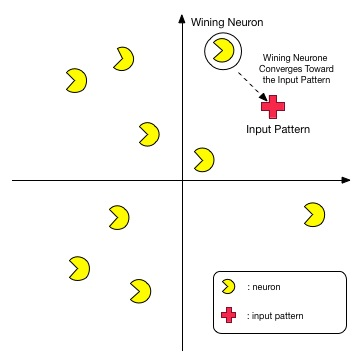
\includegraphics[width=5cm]{images/4_wining_neuron_converge.jpg}
  \end{center}
  \caption{ Winning neuron converging at learning rate }
  \label{fig:4_wining_neuron_converge}
\end{figure}

\begin{figure}
  \begin{center}
    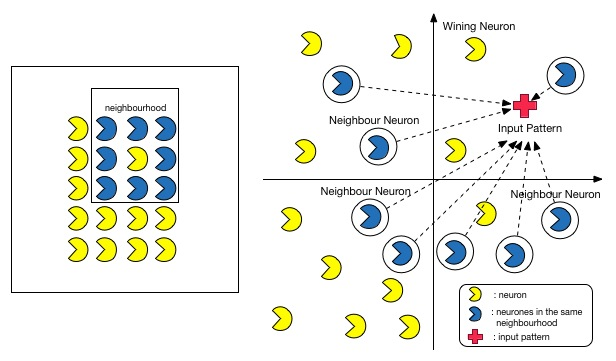
\includegraphics[width=12cm]{images/5_neighbours_converge.jpg}
  \end{center}
  \caption{ On the left the output space neighbor, on the right the neighbors of the winning neuron converging }
  \label{fig:5_neighbours_converge}
\end{figure}

After the algorithm converges, the prediction phase starts. On the prediction phase new input patterns can be quickly assigned to the SOM, without need to apply the learning rate to the winning neuron and his neighbors (the learning rate converged to zero), it very easy and fast to classify new data now. It is possible that during training the SOM gets stuck while unfolding, this kind of behavior might happen if the input patterns are very complex.

The advantages of using SOM is data noisy immunity, easy to visualize the data and parallel processing.

% subsection the_self_organizing_map (end)

